\section{Introduction}

\subsection{Remerciement}
\begin{frame}{Remerciement}
	\framesubtitle{Sans eux, ce ne sera pas possible}
	\begin{itemize}
		\item Un grand merci à M.Bouthier et M.Oster de m'avoir fait confiance et de m'avoir permis de préparer ces conférences.
		\item Un grand merci à Mme.Collin pour m'aider avec les problèmes administratifs et pour avoir accéléré la mise en place de cette leçon
		\item Merci à l'Université de Lorraine et à Télécom Nancy de m'avoir permis de préparer ces tutorats.
	\end{itemize}
\end{frame}

\subsection{À propos de moi}
\begin{frame}{À propos de moi}
	\framesubtitle{Savoir plus: \url{omarito.com}}
	\begin{columns}[T] % align columns
		\begin{column}{.71\textwidth}
			\begin{itemize}
				\item Education:
				\begin{itemize}
					\item Bac Mathématiques
					\item Licence Informatique
				\end{itemize}
				\item Premier ligne de code à l'âge de 14 ans.
				\item Grand fan de C++: 6 ans de C/C++.
				\item De nombreux projets dont un moteur de rendu, une application mobile entre autres codée en C/C++.
			\end{itemize}
		\end{column}%
		\hfill%
		\begin{column}{.25\textwidth}
			\begin{tikzpicture}[overlay,remember picture]
				\node[anchor=south east,xshift=-20pt,yshift=70pt]
				at (current page.south east) {
					
\includegraphics[width=35mm]{resources/omarito}
				};
			\end{tikzpicture}%
		\end{column}%
	\end{columns}
\end{frame}
\subsection{Organisation}
\begin{frame}{Organisation}
	\framesubtitle{Comment ça va se passer?}%
	\begin{itemize}
		\item Cours, exercices, solutions et projets seront sur \href{https://github.com/Darhal/TeachingC}{Github}.
		\item Serveur \href{https://discord.gg/y9nYQ5A5Fz}{Discord} dédié pour les questions, aide et autre.
		\item TD, TP et Projets seront en présentiel.
		\item N'hésitez pas à m'interrompre à tout moment pour poser des questions.
	\end{itemize}
\end{frame}
\subsection{L'objectif du Tutorat}

\begin{frame}{L'objectif du Tutorat}
	\begin{itemize}
		\item Vous familiariser avec la Langage C.
		\item Connaître les bonnes pratiques de programmation en C.
		\item Réussir les examens mais ça va aussi plus loin que ça.
		\item Compréhension approfondie des pointeurs et de la gestion de la mémoire en C.
		\item Bien comprendre l'outillage (Compilateur, Débogueur, autre).
	\end{itemize}
\end{frame}

\begin{frame}{L'objectif du Tutorat}
	\framesubtitle{Ce que vous pourrez faire à la fin}%
	\begin{columns}[T] % align columns
		\begin{column}{.48\textwidth}
			\begin{tikzpicture}[overlay,remember picture]
				\node[anchor=south west,xshift=10pt,yshift=70pt]
				at (current page.south west) {
					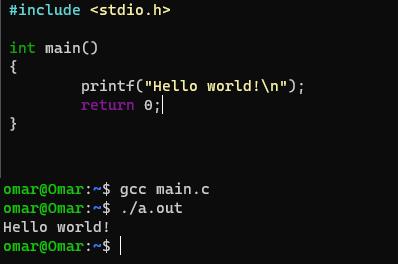
\includegraphics[scale=0.5]{resources/begin}
				};
			\end{tikzpicture}%
		\end{column}%
		%\hfill%
		\begin{column}{.065\textwidth}
			\begin{tikzpicture}[overlay,remember picture]
				\node[anchor=south west,xshift=160pt,yshift=110pt]
				at (current page.south west) {
					$\implies$
				};
			\end{tikzpicture}%
		\end{column}%
		\begin{column}{.48\textwidth}
			\begin{tikzpicture}[overlay,remember picture]
				\node[anchor=south east,xshift=-10pt,yshift=55pt]
				at (current page.south east) {
					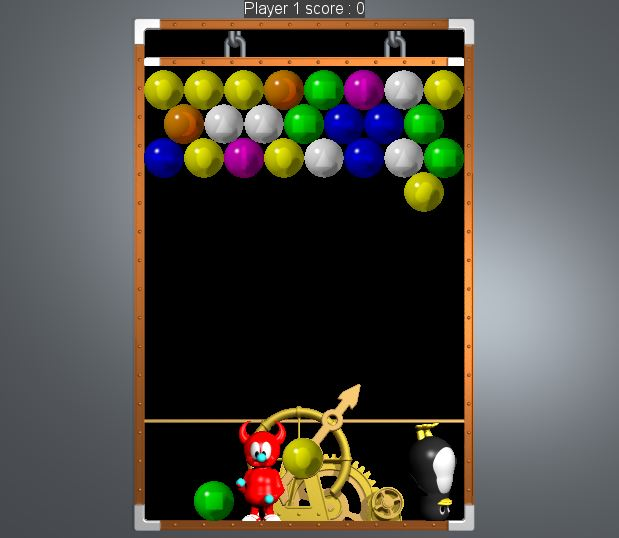
\includegraphics[scale=0.32]{resources/end}
				};
			\end{tikzpicture}%
		\end{column}%
	\end{columns}
\end{frame}

\begin{frame}{L'objectif du Tutorat}
	\framesubtitle{Ce que nous allons faire ensemble}%
	\begin{itemize}
		\item Plein d'exercices (même style que les TD).
		\begin{itemize}
			\item Exercices liés aux structures de données.
			\item Savoir des techniques intelligentes pour avoir un code C plus rapide (de l'optimisation)
		\end{itemize}
		\item Il y aura un gros projet à la fin.
		\begin{itemize}
			\item Un jeu vidéo du style (Puzzle Bobble ou Mario).
			\item Jeu sur le terminal (style Snake).
			\item Émulateur de processeur ARM.
			\item Quelque chose de plus simple que ça? (n'hésitez pas à déposer vos idées).
		\end{itemize}
	\end{itemize}
\end{frame}

\subsection{À propos de C}
\begin{frame}{À propos de C}
	\framesubtitle{Un peu de connaissances générales}%
	% dennis_ritchie
	\begin{columns}[T] % align columns
		\begin{column}{.76\textwidth}
			\begin{itemize}
				\item Langage conçu par Dennis Ritchie et développé par lui et Bell labs.
				\item Sortie en 1972 (il y a 49 ans).
				\item Utilisé dans le projet Unix développé par Dennis Ritchie et Ken Thompson entre autres.
				\item A vu une évolution relativement petite.
				\begin{itemize}
					\item K\&R C, ANSI C, C99, C11, C17, C2x.
				\end{itemize}
				\item Aujourd'hui, C est considéré comme un langage de bas niveau.
			\end{itemize}
		\end{column}%
		\hfill%
		\begin{column}{.20\textwidth}
			\begin{tikzpicture}[overlay,remember picture]
				\node[anchor=south east,xshift=-10pt,yshift=50pt]
				at (current page.south east) {
					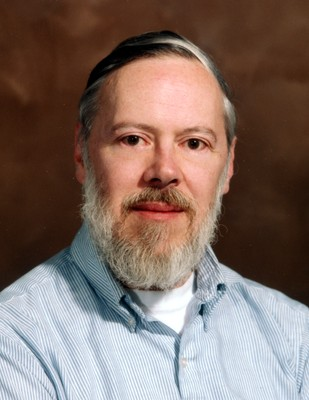
\includegraphics[width=30mm]{resources/dennis_ritchie}
				};
			\end{tikzpicture}%
		\end{column}%
	\end{columns}
\end{frame}

\subsection{Motivation : Pouquoi apprendre le C en 2021?}
\begin{frame}{Motivation : Pouquoi apprendre le C en 2021?}
	\framesubtitle{C c'est cool !}%
	\begin{itemize}
		\item C est toujours pertinent et utile aujourd'hui pour beaucoup de choses.
		\item Développement des noyaux (Kernel) et des systèmes d'exploitation
		\item Systèmes embarqués (véhicules, caméras, satellites, IoT, ...)
		\item Développement de pilotes de périphériques (Device Drivers)
		\item Bibliothèques et frameworks hautes performances (Numpy, ...)
		\item Compilateurs et interprètes de nombreuses langues populaires (Java, Python, ...).
		\item Moteurs de rendu et jeux vidéo.
		\item Bref... partout où la performance est essentielle.
	\end{itemize}
\end{frame}